\documentclass[]{book}
\usepackage{lmodern}
\usepackage{amssymb,amsmath}
\usepackage{ifxetex,ifluatex}
\usepackage{fixltx2e} % provides \textsubscript
\ifnum 0\ifxetex 1\fi\ifluatex 1\fi=0 % if pdftex
  \usepackage[T1]{fontenc}
  \usepackage[utf8]{inputenc}
\else % if luatex or xelatex
  \ifxetex
    \usepackage{mathspec}
  \else
    \usepackage{fontspec}
  \fi
  \defaultfontfeatures{Ligatures=TeX,Scale=MatchLowercase}
\fi
% use upquote if available, for straight quotes in verbatim environments
\IfFileExists{upquote.sty}{\usepackage{upquote}}{}
% use microtype if available
\IfFileExists{microtype.sty}{%
\usepackage{microtype}
\UseMicrotypeSet[protrusion]{basicmath} % disable protrusion for tt fonts
}{}
\usepackage{hyperref}
\hypersetup{unicode=true,
            pdftitle={Exploratory Analysis Project},
            pdfauthor={Matheus Amaral Mões, Marcelo Semerene Farah, Luísa Belus Henriques and Daniela de Góes N. Georg},
            pdfborder={0 0 0},
            breaklinks=true}
\urlstyle{same}  % don't use monospace font for urls
\usepackage{natbib}
\bibliographystyle{apalike}
\usepackage{color}
\usepackage{fancyvrb}
\newcommand{\VerbBar}{|}
\newcommand{\VERB}{\Verb[commandchars=\\\{\}]}
\DefineVerbatimEnvironment{Highlighting}{Verbatim}{commandchars=\\\{\}}
% Add ',fontsize=\small' for more characters per line
\usepackage{framed}
\definecolor{shadecolor}{RGB}{248,248,248}
\newenvironment{Shaded}{\begin{snugshade}}{\end{snugshade}}
\newcommand{\KeywordTok}[1]{\textcolor[rgb]{0.13,0.29,0.53}{\textbf{#1}}}
\newcommand{\DataTypeTok}[1]{\textcolor[rgb]{0.13,0.29,0.53}{#1}}
\newcommand{\DecValTok}[1]{\textcolor[rgb]{0.00,0.00,0.81}{#1}}
\newcommand{\BaseNTok}[1]{\textcolor[rgb]{0.00,0.00,0.81}{#1}}
\newcommand{\FloatTok}[1]{\textcolor[rgb]{0.00,0.00,0.81}{#1}}
\newcommand{\ConstantTok}[1]{\textcolor[rgb]{0.00,0.00,0.00}{#1}}
\newcommand{\CharTok}[1]{\textcolor[rgb]{0.31,0.60,0.02}{#1}}
\newcommand{\SpecialCharTok}[1]{\textcolor[rgb]{0.00,0.00,0.00}{#1}}
\newcommand{\StringTok}[1]{\textcolor[rgb]{0.31,0.60,0.02}{#1}}
\newcommand{\VerbatimStringTok}[1]{\textcolor[rgb]{0.31,0.60,0.02}{#1}}
\newcommand{\SpecialStringTok}[1]{\textcolor[rgb]{0.31,0.60,0.02}{#1}}
\newcommand{\ImportTok}[1]{#1}
\newcommand{\CommentTok}[1]{\textcolor[rgb]{0.56,0.35,0.01}{\textit{#1}}}
\newcommand{\DocumentationTok}[1]{\textcolor[rgb]{0.56,0.35,0.01}{\textbf{\textit{#1}}}}
\newcommand{\AnnotationTok}[1]{\textcolor[rgb]{0.56,0.35,0.01}{\textbf{\textit{#1}}}}
\newcommand{\CommentVarTok}[1]{\textcolor[rgb]{0.56,0.35,0.01}{\textbf{\textit{#1}}}}
\newcommand{\OtherTok}[1]{\textcolor[rgb]{0.56,0.35,0.01}{#1}}
\newcommand{\FunctionTok}[1]{\textcolor[rgb]{0.00,0.00,0.00}{#1}}
\newcommand{\VariableTok}[1]{\textcolor[rgb]{0.00,0.00,0.00}{#1}}
\newcommand{\ControlFlowTok}[1]{\textcolor[rgb]{0.13,0.29,0.53}{\textbf{#1}}}
\newcommand{\OperatorTok}[1]{\textcolor[rgb]{0.81,0.36,0.00}{\textbf{#1}}}
\newcommand{\BuiltInTok}[1]{#1}
\newcommand{\ExtensionTok}[1]{#1}
\newcommand{\PreprocessorTok}[1]{\textcolor[rgb]{0.56,0.35,0.01}{\textit{#1}}}
\newcommand{\AttributeTok}[1]{\textcolor[rgb]{0.77,0.63,0.00}{#1}}
\newcommand{\RegionMarkerTok}[1]{#1}
\newcommand{\InformationTok}[1]{\textcolor[rgb]{0.56,0.35,0.01}{\textbf{\textit{#1}}}}
\newcommand{\WarningTok}[1]{\textcolor[rgb]{0.56,0.35,0.01}{\textbf{\textit{#1}}}}
\newcommand{\AlertTok}[1]{\textcolor[rgb]{0.94,0.16,0.16}{#1}}
\newcommand{\ErrorTok}[1]{\textcolor[rgb]{0.64,0.00,0.00}{\textbf{#1}}}
\newcommand{\NormalTok}[1]{#1}
\usepackage{longtable,booktabs}
\usepackage{graphicx,grffile}
\makeatletter
\def\maxwidth{\ifdim\Gin@nat@width>\linewidth\linewidth\else\Gin@nat@width\fi}
\def\maxheight{\ifdim\Gin@nat@height>\textheight\textheight\else\Gin@nat@height\fi}
\makeatother
% Scale images if necessary, so that they will not overflow the page
% margins by default, and it is still possible to overwrite the defaults
% using explicit options in \includegraphics[width, height, ...]{}
\setkeys{Gin}{width=\maxwidth,height=\maxheight,keepaspectratio}
\IfFileExists{parskip.sty}{%
\usepackage{parskip}
}{% else
\setlength{\parindent}{0pt}
\setlength{\parskip}{6pt plus 2pt minus 1pt}
}
\setlength{\emergencystretch}{3em}  % prevent overfull lines
\providecommand{\tightlist}{%
  \setlength{\itemsep}{0pt}\setlength{\parskip}{0pt}}
\setcounter{secnumdepth}{5}
% Redefines (sub)paragraphs to behave more like sections
\ifx\paragraph\undefined\else
\let\oldparagraph\paragraph
\renewcommand{\paragraph}[1]{\oldparagraph{#1}\mbox{}}
\fi
\ifx\subparagraph\undefined\else
\let\oldsubparagraph\subparagraph
\renewcommand{\subparagraph}[1]{\oldsubparagraph{#1}\mbox{}}
\fi

%%% Use protect on footnotes to avoid problems with footnotes in titles
\let\rmarkdownfootnote\footnote%
\def\footnote{\protect\rmarkdownfootnote}

%%% Change title format to be more compact
\usepackage{titling}

% Create subtitle command for use in maketitle
\providecommand{\subtitle}[1]{
  \posttitle{
    \begin{center}\large#1\end{center}
    }
}

\setlength{\droptitle}{-2em}

  \title{Exploratory Analysis Project}
    \pretitle{\vspace{\droptitle}\centering\huge}
  \posttitle{\par}
    \author{Matheus Amaral Mões, Marcelo Semerene Farah, Luísa Belus Henriques and
Daniela de Góes N. Georg}
    \preauthor{\centering\large\emph}
  \postauthor{\par}
      \predate{\centering\large\emph}
  \postdate{\par}
    \date{2019-09-15}

\usepackage{booktabs}

\begin{document}
\maketitle

{
\setcounter{tocdepth}{1}
\tableofcontents
}
\chapter{Introduction}\label{introduction}

This project is part of the Exploratory Data Analysis discipline of the
Getulio Vargas Foundation in Business Analytics and Big Data MBA.
Members of the group: Matheus Amaral Mões, Marcelo Semerene Farah, Luísa
Belus Henriques and Daniela de Góes N. Georg

Context and objective The manager of a Czech bank wants to get a better
understanding on his clients. To do so, it has an extensive database
that records customers and their transactions as follows:

To assist the manager, our team works with the database in the following
steps: Understand, clean and organize data; Search relationships between
data; Find product and service opportunities for the bank.

To assist the manager, our team worked with the database in the
following steps:

\begin{enumerate}
\def\labelenumi{\arabic{enumi}.}
\item
  Understand, clean and organize data;
\item
  Search relationships between data;
\item
  Find product and service opportunities for the bank.
\end{enumerate}

This book is organized according to the steps taken to reach a
conclusion about the clients.

\chapter{Read Files}\label{read-files}

The first step was to read the files and organize them. In each file,
some columns had to be translated and some data reordered to facilitate
the exploratory analysis work.

\begin{figure}
\centering
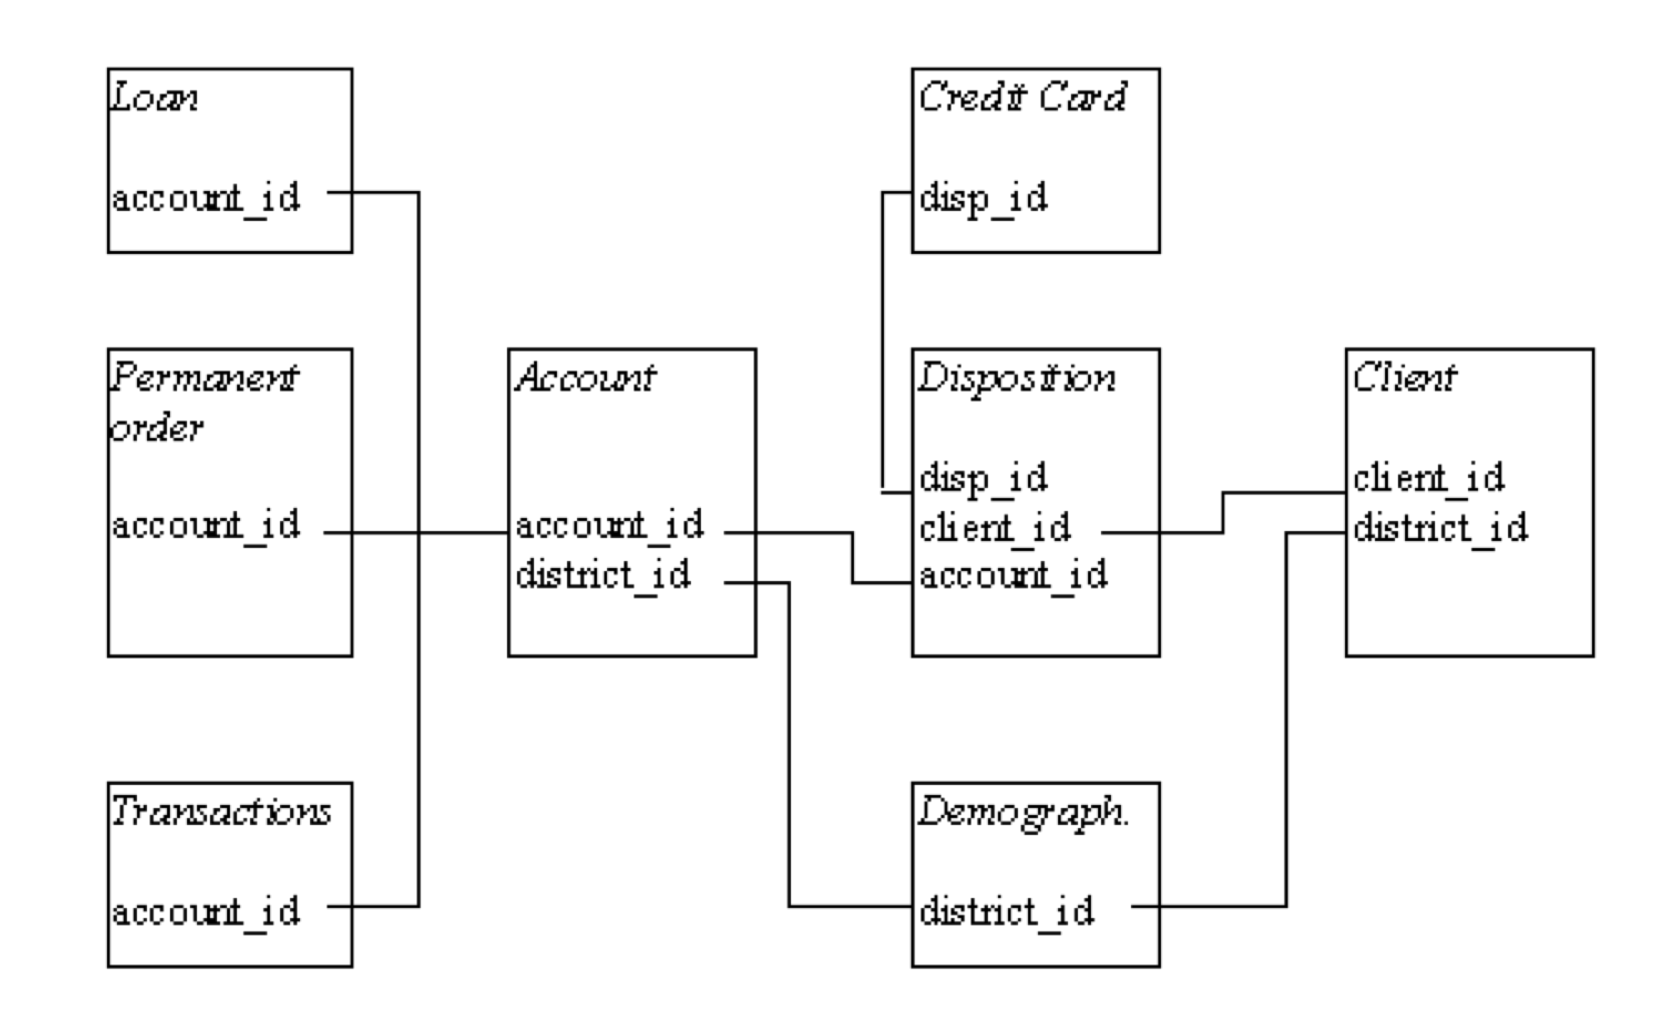
\includegraphics{dados.png}
\caption{data}
\end{figure}

\section{Accounts}\label{accounts}

Here we find the account data. There are 4500 records, each containing
information about the account district, frequency of statement issuance,
and date of account creation.

To make the data easier to understand, we translate Czech frequency
values into English and separate dates with hyphens.

\begin{table}[t]

\caption{\label{tab:unnamed-chunk-4}accounts frame}
\centering
\begin{tabular}{r|r|l|l}
\hline
account\_id & district\_id & frequency & date\\
\hline
576 & 55 & monthly & 1993-01-01\\
\hline
3818 & 74 & monthly & 1993-01-01\\
\hline
704 & 55 & monthly & 1993-01-01\\
\hline
2378 & 16 & monthly & 1993-01-01\\
\hline
2632 & 24 & monthly & 1993-01-02\\
\hline
\end{tabular}
\end{table}

\section{Clients}\label{clients}

The Clients list contains 5369 bank customers, tabulated with the
district code and their birthday code - which informs the birthday and
gender. For the analysis, we separated the date of birth and gender in
separate columns.

\begin{table}[t]

\caption{\label{tab:unnamed-chunk-5}clients frame}
\centering
\begin{tabular}{r|r|r|r|l|l}
\hline
client\_id & birth\_number & district\_id & gender\_code & gender & birth\_date\\
\hline
1 & 706213 & 18 & 1 & W & 1970-12-13\\
\hline
2 & 450204 & 1 & 0 & M & 1945-02-04\\
\hline
3 & 406009 & 1 & 1 & W & 1940-10-09\\
\hline
4 & 561201 & 5 & 0 & M & 1956-12-01\\
\hline
5 & 605703 & 5 & 1 & W & 1960-07-03\\
\hline
\end{tabular}
\end{table}

\section{Disposition}\label{disposition}

The Disposition relationship contains interactions between customers and
accounts, classifying as owner / dependent. Some explanations of
possible account-owner-dependency interactions: Every account has an
owner and may or may not have dependents. Dependents may own another
account. A customer may own more than one account.

\begin{table}[t]

\caption{\label{tab:unnamed-chunk-6}disposition frame}
\centering
\begin{tabular}{r|r|r|l}
\hline
disp\_id & client\_id & account\_id & type\\
\hline
1 & 1 & 1 & OWNER\\
\hline
2 & 2 & 2 & OWNER\\
\hline
3 & 3 & 2 & DISPONENT\\
\hline
4 & 4 & 3 & OWNER\\
\hline
5 & 5 & 3 & DISPONENT\\
\hline
\end{tabular}
\end{table}

\section{Order}\label{order}

List of payment orders issued to accounts. In addition to the money
order code and the account code, the records contain information about
the bank and account you received, the amount and type of payment
(household, insurance, leasing and loan). To make it easier to
understand, it was necessary to translate Czech payment types into
English.

\begin{table}[t]

\caption{\label{tab:unnamed-chunk-7}order frame}
\centering
\begin{tabular}{r|r|l|r|r|l}
\hline
order\_id & account\_id & bank\_to & account\_to & amount & k\_symbol\\
\hline
29401 & 1 & YZ & 87144583 & 2452.0 & household\\
\hline
29402 & 2 & ST & 89597016 & 3372.7 & loan\\
\hline
29403 & 2 & QR & 13943797 & 7266.0 & household\\
\hline
29404 & 3 & WX & 83084338 & 1135.0 & household\\
\hline
29405 & 3 & CD & 24485939 & 327.0 & \\
\hline
\end{tabular}
\end{table}

\section{Transactions}\label{transactions}

List of all transactions made by customers, informing: Account that
performed the transaction Transaction Date Transaction Type (Inbound and
Outbound) Transaction (credit card withdrawal, credit in cash,
collection from another bank, withdrawal in cash, remittance to another
bank) Amount (transaction amount) Balance after transaction K-symbol
(characterization of transaction) Bank (receiving bank) Account
(receiving account)

\begin{table}[t]

\caption{\label{tab:unnamed-chunk-8}transaction frame}
\centering
\begin{tabular}{r|r|l|l|l|r|r|l|l|r}
\hline
trans\_id & account\_id & date & type & operation & amount & balance & k\_symbol & bank & account\\
\hline
695247 & 2378 & 1993-01-01 & credit & credit in cash & 700 & 700 &  &  & NA\\
\hline
171812 & 576 & 1993-01-01 & credit & credit in cash & 900 & 900 &  &  & NA\\
\hline
207264 & 704 & 1993-01-01 & credit & credit in cash & 1000 & 1000 &  &  & NA\\
\hline
1117247 & 3818 & 1993-01-01 & credit & credit in cash & 600 & 600 &  &  & NA\\
\hline
579373 & 1972 & 1993-01-02 & credit & credit in cash & 400 & 400 &  &  & NA\\
\hline
\end{tabular}
\end{table}

\section{Loans}\label{loans}

Loan list, with 682 occurrences. Each customer can only receive one
loan. In the table we have Loan key Account Key Date Value Duration (in
months) Installment Payment Amount Status (finished - ok; Finished - not
ok; Running - ok; Running - in debt) To make understanding easier during
the analysis, we classify the status according to its conditions rather
than leaving the original groups A through D from the database.

\begin{table}[t]

\caption{\label{tab:unnamed-chunk-9}loan frame}
\centering
\begin{tabular}{r|r|l|r|r|r|l}
\hline
loan\_id & account\_id & date & amount & duration & payments & status\\
\hline
5314 & 1787 & 1993-07-05 & 96396 & 12 & 8033 & Finished - not payed\\
\hline
5316 & 1801 & 1993-07-11 & 165960 & 36 & 4610 & Finished - OK\\
\hline
6863 & 9188 & 1993-07-28 & 127080 & 60 & 2118 & Finished - OK\\
\hline
5325 & 1843 & 1993-08-03 & 105804 & 36 & 2939 & Finished - OK\\
\hline
7240 & 11013 & 1993-09-06 & 274740 & 60 & 4579 & Finished - OK\\
\hline
\end{tabular}
\end{table}

\section{Credit Card}\label{credit-card}

The credit card list contains 892 occurrences and stores the card code,
disposition id, card type (junior / classic / gold) and date of issue.
Treatment was performed so that the issue date was in the Brazilian
model.

\begin{table}[t]

\caption{\label{tab:unnamed-chunk-10}card frame}
\centering
\begin{tabular}{r|r|l|l}
\hline
card\_id & disp\_id & type & issued\\
\hline
1005 & 9285 & classic & 1993-11-07\\
\hline
104 & 588 & classic & 1994-01-19\\
\hline
747 & 4915 & classic & 1994-02-05\\
\hline
70 & 439 & classic & 1994-02-08\\
\hline
577 & 3687 & classic & 1994-02-15\\
\hline
\end{tabular}
\end{table}

\section{Demographic data}\label{demographic-data}

Finally, demographic data records 77 municipalities distributed in the 7
regions of the Czech Republic. The table contains the following
elements:

District code;

District name;

Region;

Nº of inhabitants

Nº of municipalities with \textless{}499 inhabitants

Nº of municipalities with 500-1999 inhabitants

Nº of municipalities with 2000-9999 inhabitants

Nº of municipalities with\textgreater{} 1000 inhabitants

Nº of cities

Proportion of urban inhabitants

Average Salary

unemployment rate `95

Unemployment Rate `96

Nº of entrepreneurs per 1000 inhabitants

Nº of crimes committed in `95

Nº of crimes committed in `96

\begin{table}[t]

\caption{\label{tab:unnamed-chunk-11}demographic frame}
\centering
\begin{tabular}{l|l|r}
\hline
region & district\_name & inhabitants\\
\hline
Prague & Hl.m. Praha & 1204953\\
\hline
central Bohemia & Benesov & 88884\\
\hline
central Bohemia & Beroun & 75232\\
\hline
central Bohemia & Kladno & 149893\\
\hline
central Bohemia & Kolin & 95616\\
\hline
\end{tabular}
\end{table}

\chapter{Join Frames}\label{join-frames}

In order to explore our database, we decided to combine the different
tables. This was a two-step process:

\begin{enumerate}
\def\labelenumi{\arabic{enumi}.}
\item
  Aggregate every table but the transactions in which the granularity
  was the account, the clients were agregated to show only the account
  owner and the number of the dependants in the account.
\item
  Next step was to join this new table with Transactions, creating a big
  dataset with all the data. The granularity for this is the single
  transaction.
\end{enumerate}

With this two new structures we were able to study the data and draw
some ideas and conclusions to help the manager.

\section{Join frames without
transactions:}\label{join-frames-without-transactions}

\begin{Shaded}
\begin{Highlighting}[]
\CommentTok{#Base frame accounts }
\NormalTok{frame_no_transaction <-}\StringTok{ }\NormalTok{account }\OperatorTok
\StringTok{  }\CommentTok{#Join accounts}
\StringTok{  }\KeywordTok{left_join}\NormalTok{(loan, }\DataTypeTok{by =} \StringTok{'account_id'}\NormalTok{) }\OperatorTok
\StringTok{  }\CommentTok{#Join Demographic}
\StringTok{  }\KeywordTok{left_join}\NormalTok{(demographic, }\DataTypeTok{by =} \StringTok{'district_id'}\NormalTok{) }\OperatorTok
\StringTok{  }\CommentTok{#Join disposition}
\StringTok{  }\KeywordTok{left_join}\NormalTok{(}
\NormalTok{    dplyr}\OperatorTok{::}\KeywordTok{filter}\NormalTok{(disposition, type }\OperatorTok{==}\StringTok{ 'OWNER'}\NormalTok{ ) }\OperatorTok\StringTok{ }
\StringTok{      }\KeywordTok{left_join}\NormalTok{(disposition }\OperatorTok\StringTok{ }\KeywordTok{group_by}\NormalTok{(account_id) }\OperatorTok\StringTok{ }
\StringTok{                  }\NormalTok{dplyr}\OperatorTok{::}\KeywordTok{summarise}\NormalTok{(}\DataTypeTok{dependents =} \KeywordTok{n}\NormalTok{()}\OperatorTok{-}\DecValTok{1}\NormalTok{), }\DataTypeTok{by =} \StringTok{'account_id'}\NormalTok{)}
\NormalTok{    , }\DataTypeTok{by =} \StringTok{'account_id'}\NormalTok{) }\OperatorTok
\StringTok{  }\CommentTok{#Join client}
\StringTok{  }\KeywordTok{left_join}\NormalTok{(client,}\DataTypeTok{by =} \StringTok{'client_id'}\NormalTok{) }\OperatorTok
\StringTok{  }\CommentTok{#Join card}
\StringTok{  }\KeywordTok{left_join}\NormalTok{(card, }\DataTypeTok{by =} \StringTok{'disp_id'}\NormalTok{) }\OperatorTok
\StringTok{  }\CommentTok{#Join order}
\StringTok{  }\KeywordTok{left_join}\NormalTok{(order, }\DataTypeTok{by =} \StringTok{'account_id'}\NormalTok{) }\OperatorTok
\StringTok{  }\CommentTok{#Join transactions }
\StringTok{  }\KeywordTok{left_join}\NormalTok{(}
\NormalTok{    transaction }\OperatorTok\StringTok{ }\KeywordTok{group_by}\NormalTok{(account_id) }\OperatorTok
\StringTok{      }\NormalTok{dplyr}\OperatorTok{::}\KeywordTok{summarise}\NormalTok{(}\DataTypeTok{amount_transactions =} \KeywordTok{sum}\NormalTok{(amount)),}
    \DataTypeTok{by =} \StringTok{'account_id'}\NormalTok{)}
\end{Highlighting}
\end{Shaded}

\section{Join frames with
transactions:}\label{join-frames-with-transactions}

\begin{Shaded}
\begin{Highlighting}[]
\CommentTok{# Join previous frame with transactions}
\NormalTok{frame <-}\StringTok{ }\NormalTok{transaction }\OperatorTok
\StringTok{  }\KeywordTok{left_join}\NormalTok{(frame_no_transaction, }\DataTypeTok{by =} \StringTok{'account_id'}\NormalTok{)}
\end{Highlighting}
\end{Shaded}

\chapter{Client Profile}\label{client-profile}

Understanding who the customer is is a critical step in generating
hypotheses and moving on with the analysis. To do this, we explored the
data and found some interesting information shared below:

\section{Birth Date}\label{birth-date}

The majority of the bank's clients were born after the 40s.
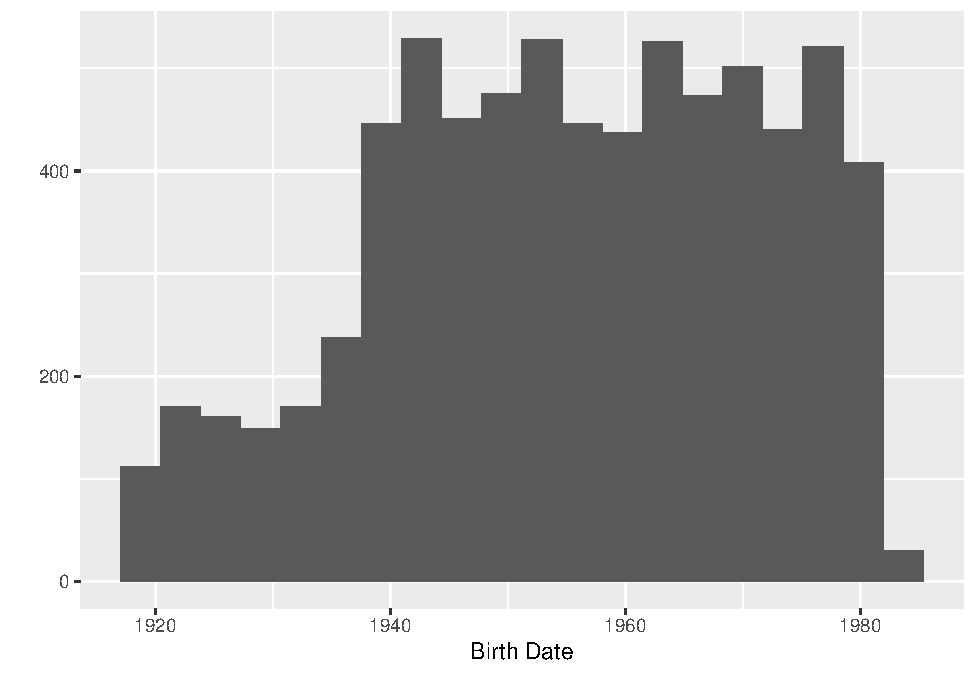
\includegraphics{bookdown_files/figure-latex/unnamed-chunk-18-1.pdf}
\#\#Gender

There is a close distribution between male and female clients in the
bank.
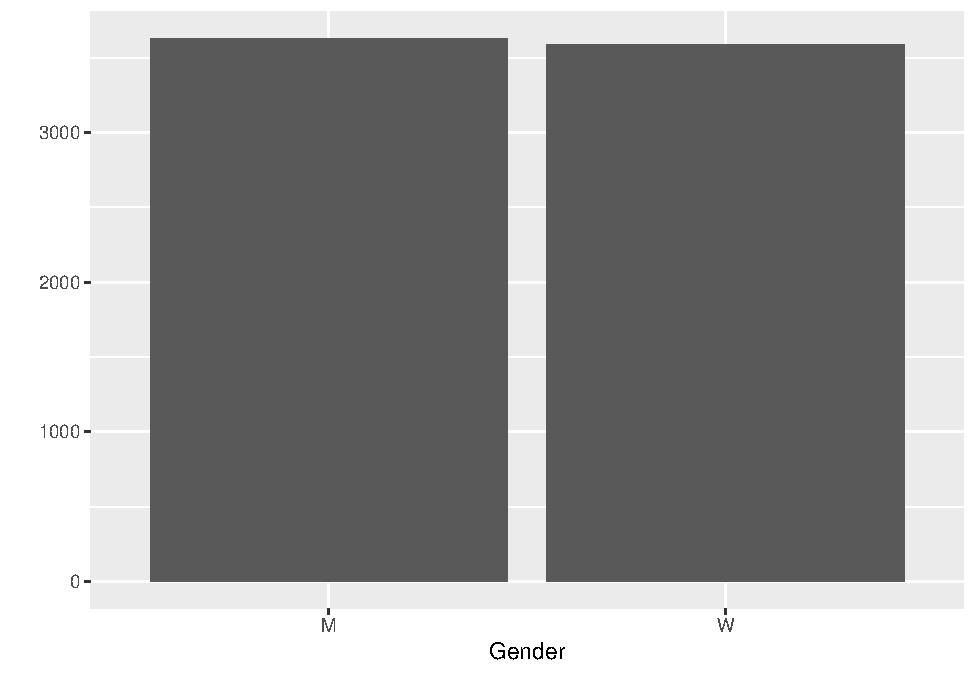
\includegraphics{bookdown_files/figure-latex/unnamed-chunk-19-1.pdf}

\section{Number of Dependents}\label{number-of-dependents}

Most of the bank's clients don't have any dependents on their bank and
account and the ones that do, only have one dependant. If having
dependents is a revenue stream of the bank, this should be taken into
consideration as an opportunity to grow.

\begin{figure}
\centering
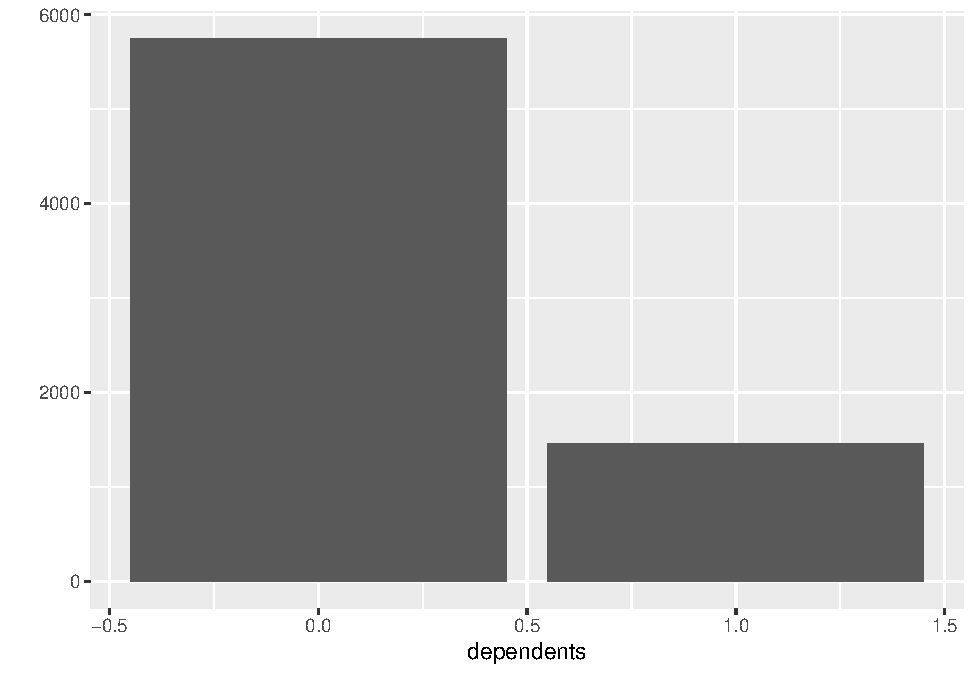
\includegraphics{bookdown_files/figure-latex/unnamed-chunk-20-1.pdf}
\caption{\label{fig:unnamed-chunk-20}Number of Dependents}
\end{figure}

\section{Account creation by time}\label{account-creation-by-time}

There was a sharp decrease in accounts created after 1994 and since then
the bank has been recovering from it.

Recommendation: investigate the root causes on this decrease, this way
the bank can become aware of what impacts it's business.

\begin{figure}
\centering
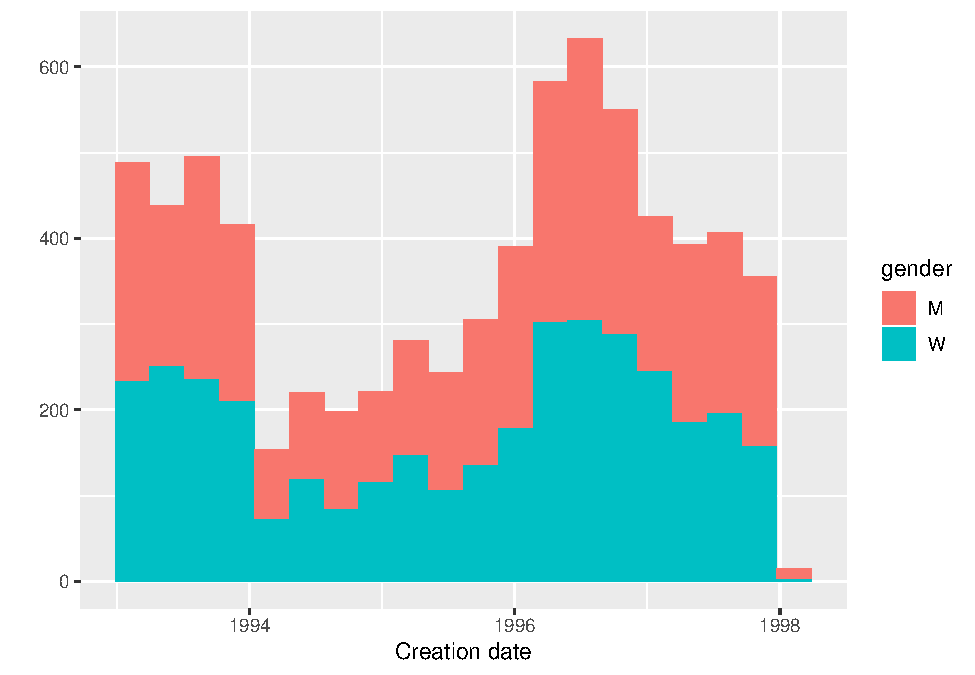
\includegraphics{bookdown_files/figure-latex/unnamed-chunk-21-1.pdf}
\caption{\label{fig:unnamed-chunk-21}Distribution of birth date}
\end{figure}

\section{Age at account creation}\label{age-at-account-creation}

The youngest clients that the bank manage to capitate are on their late
teens when they create their bank account and there is a sharp decrease
of account creation after the 60s.

Having young clients is great for the business in the long term, but
they are usually not as profitable as older clients (who already have
higher incomes and do more bank transactions). It is suggested to seek
greater penetration in the elderly market.

\begin{figure}
\centering
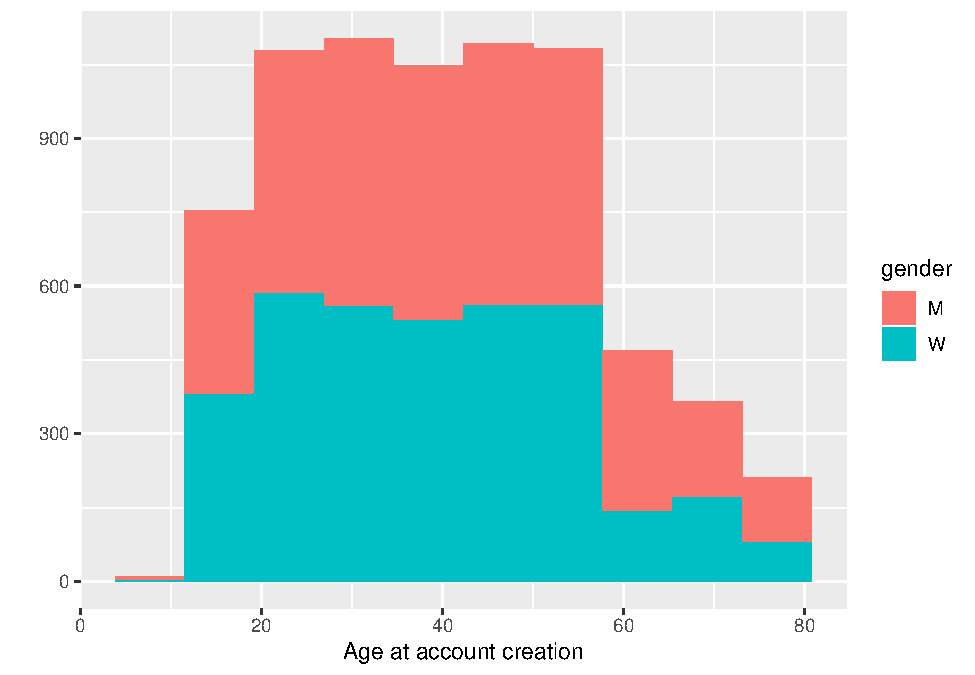
\includegraphics{bookdown_files/figure-latex/unnamed-chunk-22-1.pdf}
\caption{\label{fig:unnamed-chunk-22}Distribution of birth date}
\end{figure}

\section{Regions}\label{regions}

There is no concentration of clients in any particular region in the
country.

Given this scenario, a possible strategy would be to focus on some more
profitable regions and gain space in them, then expand and gain more
customers in all regions.

\begin{figure}
\centering
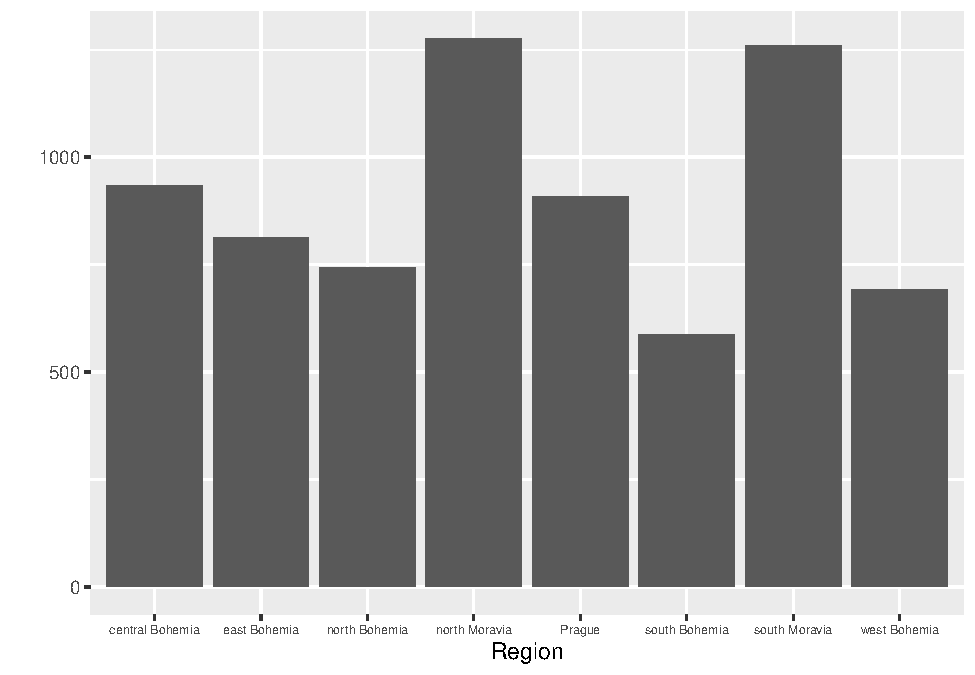
\includegraphics{bookdown_files/figure-latex/unnamed-chunk-23-1.pdf}
\caption{\label{fig:unnamed-chunk-23}Clients by Region}
\end{figure}

Looking closely to number of inhabitants in each region and the number
of clients we see that there is a major opportunity for improvement in
South Moravia.

\begin{figure}
\centering
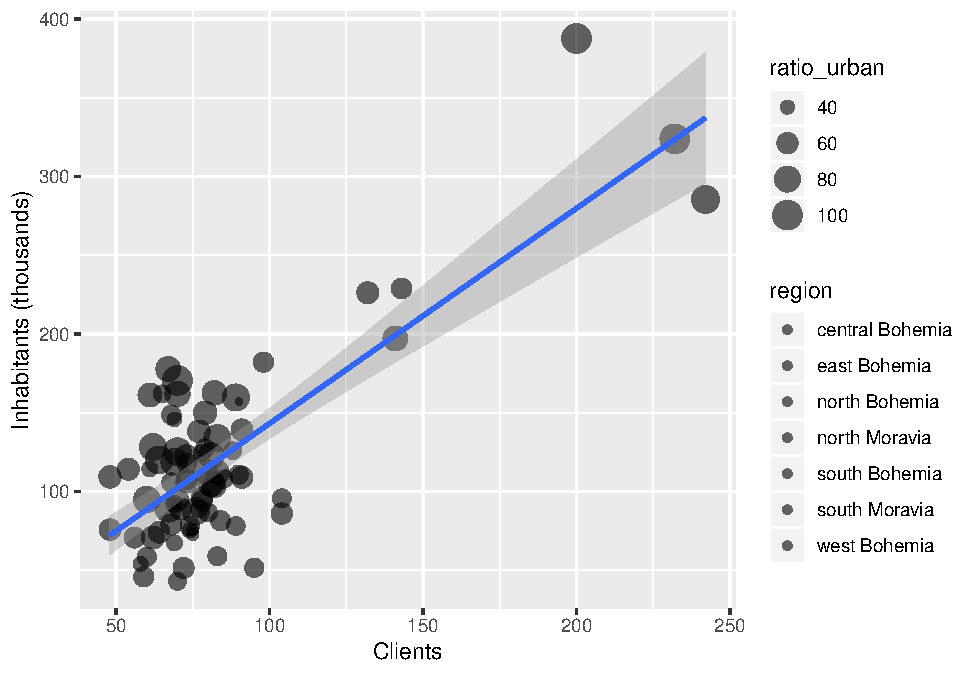
\includegraphics{bookdown_files/figure-latex/unnamed-chunk-24-1.pdf}
\caption{\label{fig:unnamed-chunk-24}Clients by Region}
\end{figure}

\section{Frequency of statements}\label{frequency-of-statements}

Almost all clients prefer to have their bank statements sent to them
monthly.

\begin{figure}
\centering
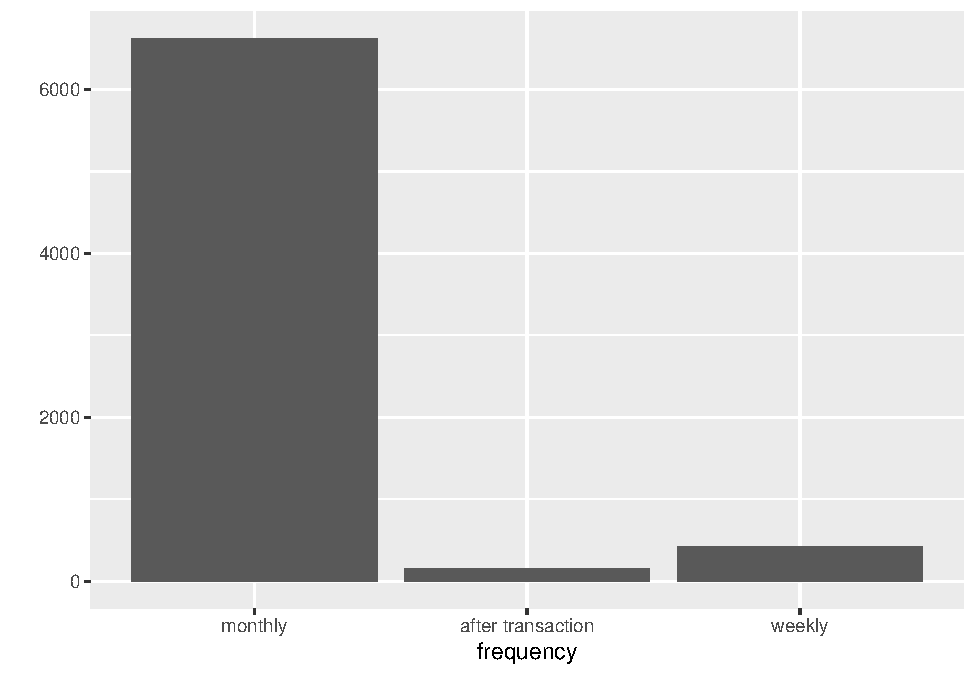
\includegraphics{bookdown_files/figure-latex/unnamed-chunk-25-1.pdf}
\caption{\label{fig:unnamed-chunk-25}Frequency of statements}
\end{figure}

No bank client born before the 30s choose to have its bank statement
sent after transaction or weekly.

\begin{figure}
\centering
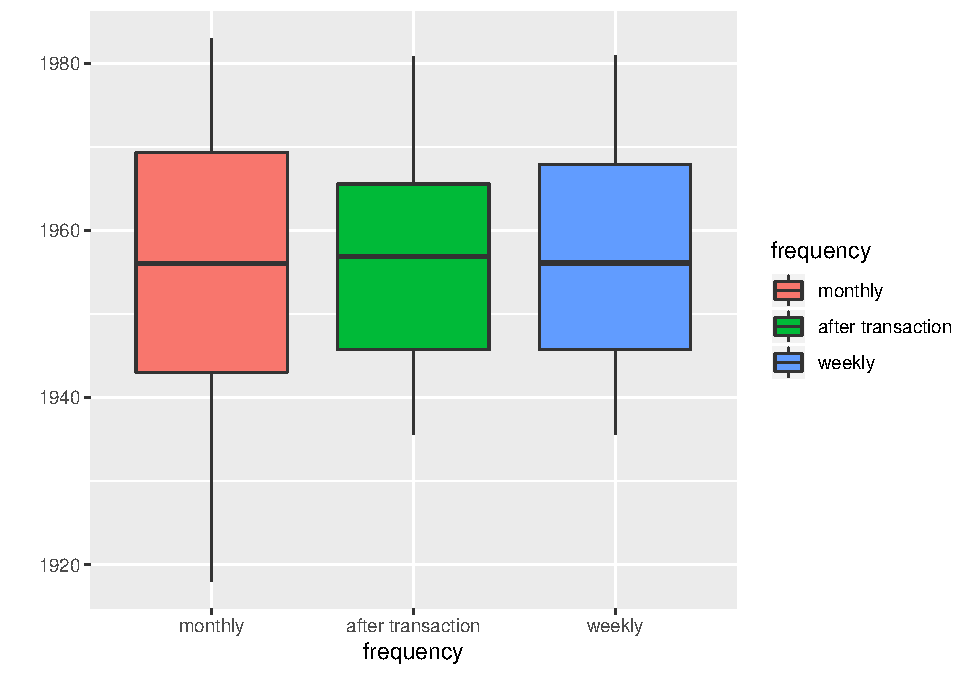
\includegraphics{bookdown_files/figure-latex/unnamed-chunk-26-1.pdf}
\caption{\label{fig:unnamed-chunk-26}Frequency of statements}
\end{figure}

\chapter{Loans}\label{loans-1}

Loans are a great source of revenue for the bank, so we look at data for
opportunities and outlier patterns.

\section{Loans Status}\label{loans-status}

The bank currently has a healthy record of loans with the majority of
loans finished being paid correctly and less then 15\% not being paid
back. The current loans are also in good state with the majority of
those running without problems and aproximatly 10\% with the client in
debt.

As the numbers indicate that the credit division is doing well in
selecting their clients, it is suggested to extend the possibility of
extending this lending to clients with similar profiles to borrowers.
Accordingly, we may increase our profits from the volume of such
interest.

\begin{figure}
\centering
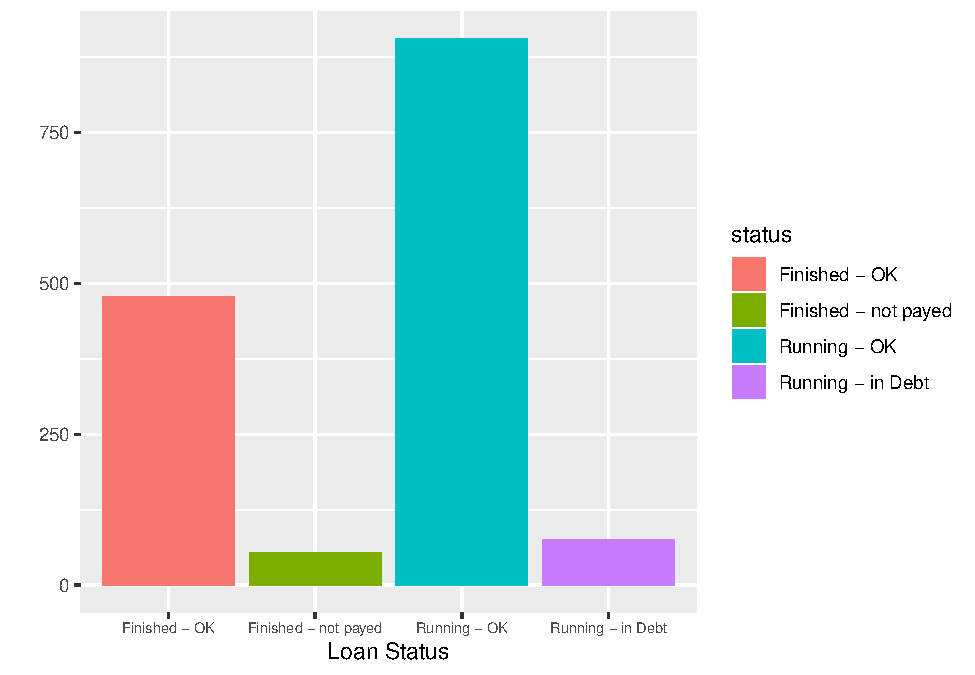
\includegraphics{bookdown_files/figure-latex/unnamed-chunk-28-1.pdf}
\caption{\label{fig:unnamed-chunk-28}Loan Status}
\end{figure}

We can also see that that the number of loans with some problem does not
appear to have a growing tendency, although we can see that there is a
decline in loans being issued by the bank in 1998 showing some room for
improvement. Also in 1997 there was a great number of bad loans,
problaby being the caus for the reduction of loans in 1998.

\begin{figure}
\centering
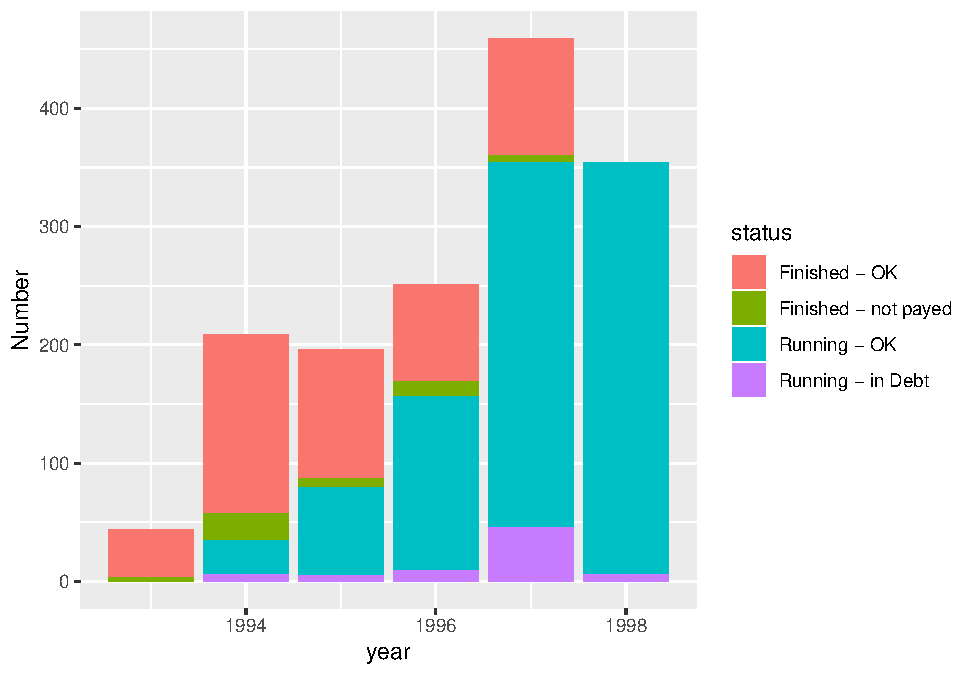
\includegraphics{bookdown_files/figure-latex/unnamed-chunk-29-1.pdf}
\caption{\label{fig:unnamed-chunk-29}Loan status by creation date}
\end{figure}

\section{Age distributions of loan}\label{age-distributions-of-loan}

We can see that the bank spreads its loan through different age groups
with the bulk of loans occurring from the 20s to the late 50s of its
costumers and there is no major concentration of bad loans in any age
group.

\begin{figure}
\centering
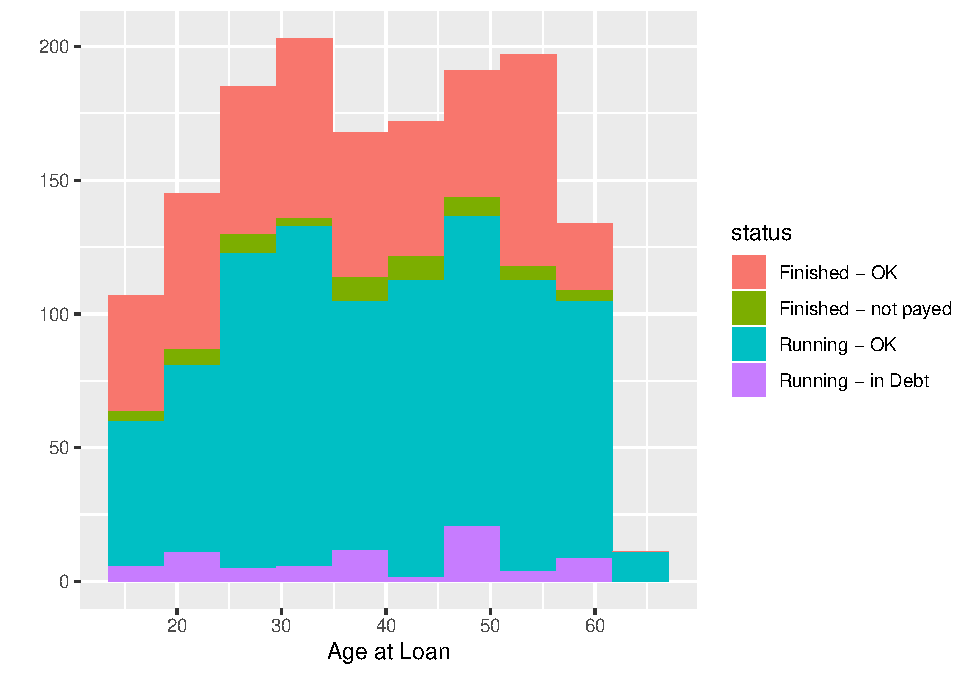
\includegraphics{bookdown_files/figure-latex/unnamed-chunk-30-1.pdf}
\caption{\label{fig:unnamed-chunk-30}Loans by birth date}
\end{figure}

By the Boxplot we can confirm the same conclusions with the addition
that loans finished and not payed happened more with slighlty older
people than the others.

\begin{figure}
\centering
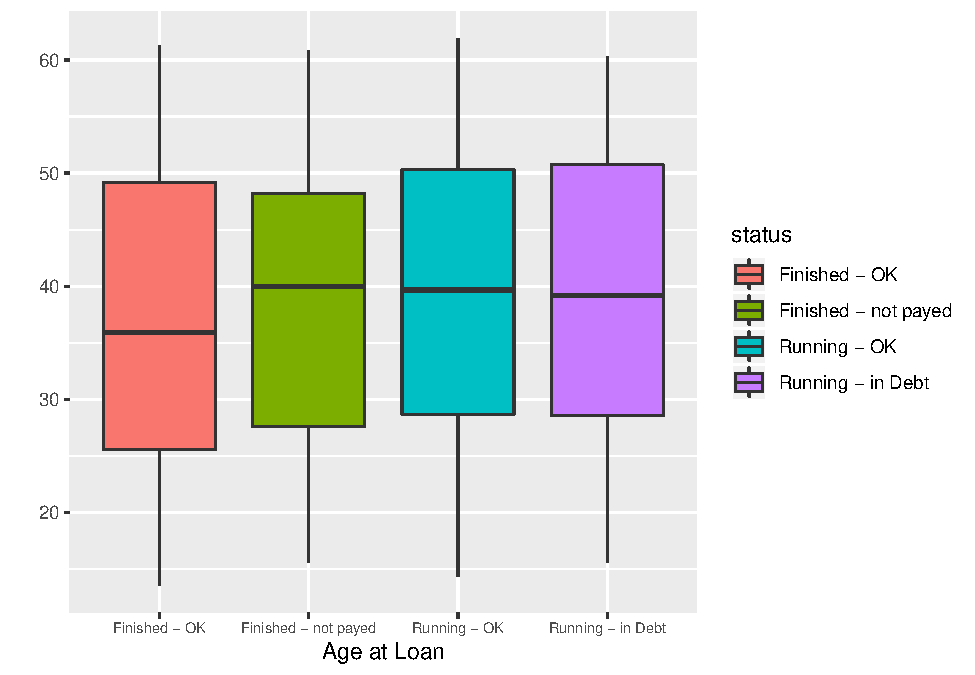
\includegraphics{bookdown_files/figure-latex/unnamed-chunk-31-1.pdf}
\caption{\label{fig:unnamed-chunk-31}Boxplot loans by birth date}
\end{figure}

\section{Loans status by size of
loan}\label{loans-status-by-size-of-loan}

Analyzing the number size of loans taken we can see that bigger loans
have higher risks. Comparing the loans finished and the ones still
running we can see that in both groups there is ones with problems have
a higher median value. Also with we can see that ther is a great number
of outliers in the analysis.

By this information, is suggested to focus on bigger volumes of small
loans, so the bank can make profit from it with less risk.

\begin{figure}
\centering
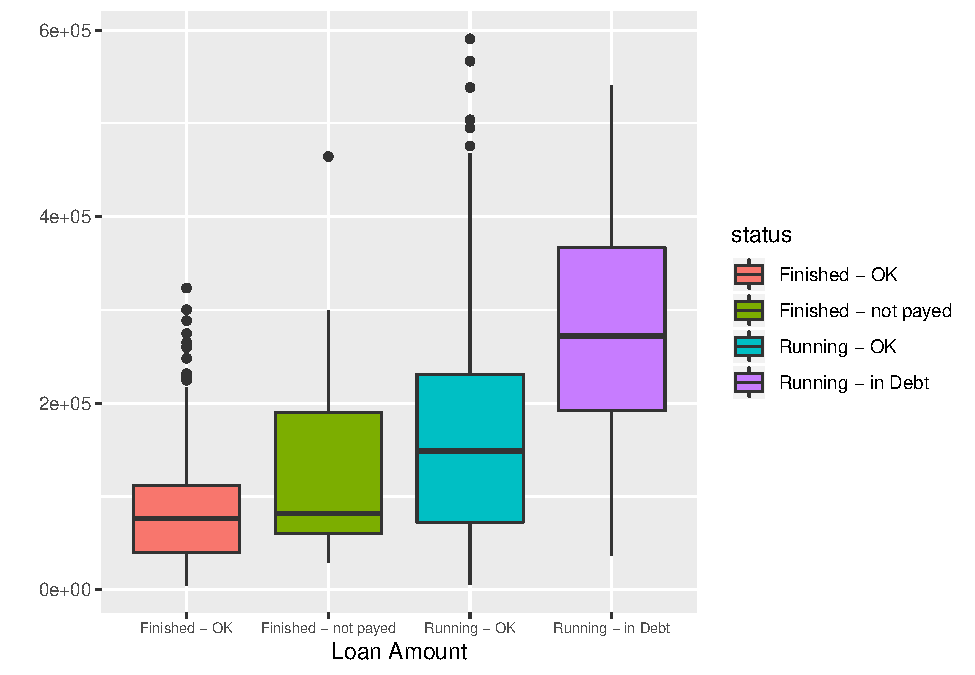
\includegraphics{bookdown_files/figure-latex/unnamed-chunk-32-1.pdf}
\caption{\label{fig:unnamed-chunk-32}Distribution of birth date}
\end{figure}

\section{Loans status by monthly
payment}\label{loans-status-by-monthly-payment}

The number of outliers previously seen can be explained by the loans
with a larger duration, in an analysis of loan size divided by duration
we can see that there are no outliers in the boxplot. That analysis also
shows that there are more problems in the loans with the higher monthly
payment, so focusing on smaller loans could be a better strategy for the
company. An interesting insight is that currently there is no default in
the loans with a monthly payment smaller then 1.670 so the bank could be
more agressive on those loans.

\begin{figure}
\centering
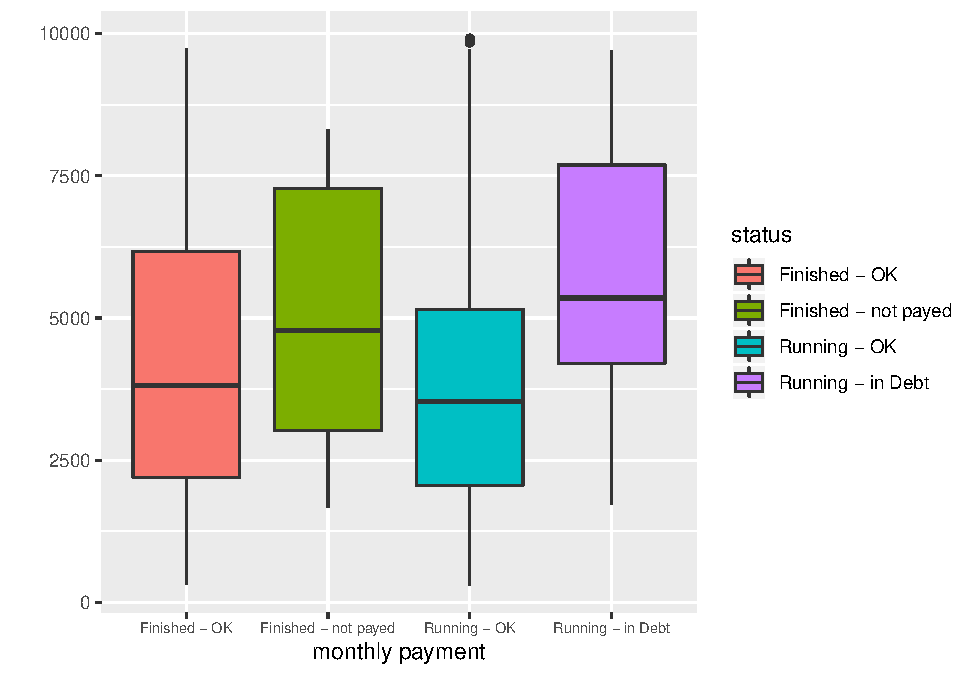
\includegraphics{bookdown_files/figure-latex/unnamed-chunk-33-1.pdf}
\caption{\label{fig:unnamed-chunk-33}Loans status by monthly payment}
\end{figure}

\chapter{Transactions}\label{transactions-1}

\section{Amount of transactions
annually}\label{amount-of-transactions-annually}

The amount of transactions done by the bank is growing continuously,
showing the bank's growth. The majority of those transactions involves
physical cash, either withdrawal or credit, and those are the most
important drivers in the transaction's growth. The share of credit card
in the banks transactions is very small.

This indicates an opportunity of growth from offering more credit cards
and making incentives for the clients to use them.

\begin{figure}
\centering
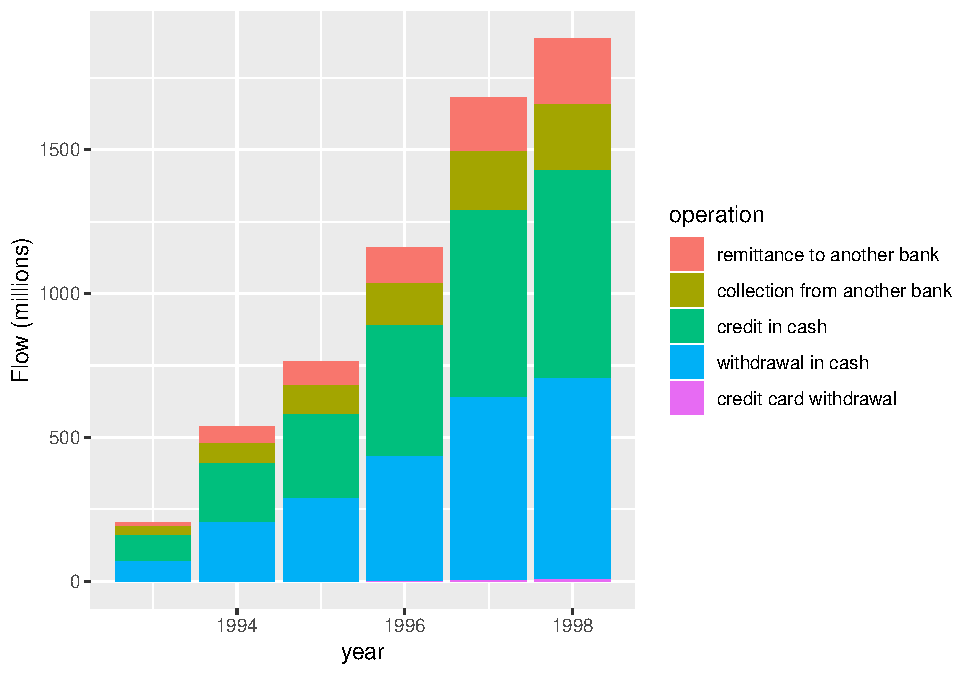
\includegraphics{bookdown_files/figure-latex/unnamed-chunk-35-1.pdf}
\caption{\label{fig:unnamed-chunk-35}Amount of transactions annually}
\end{figure}

\section{Net transactions amount
annually}\label{net-transactions-amount-annually}

We can see that in every year on the time series the net flow of
transactions is positive, which indicates that the bank shouldn't have a
liquidity problem.

\begin{figure}
\centering
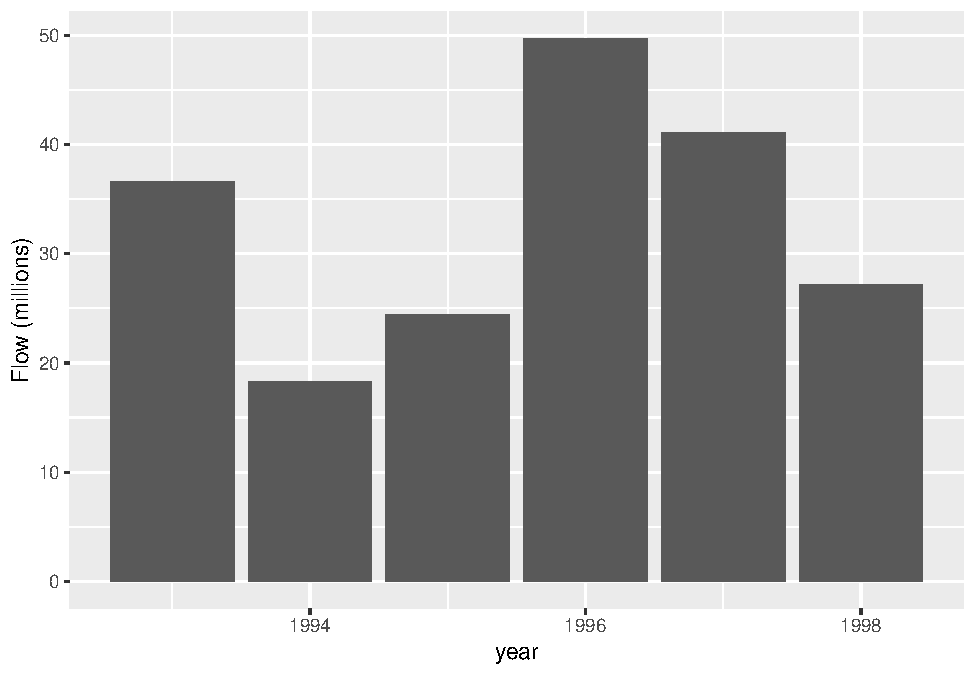
\includegraphics{bookdown_files/figure-latex/unnamed-chunk-36-1.pdf}
\caption{\label{fig:unnamed-chunk-36}Net transactions amount annually}
\end{figure}

\section{Net transactions amount
monthly}\label{net-transactions-amount-monthly}

If we take a closer look to the transactions monthly, we can that on
every January and June of every year there is a negative flow of
transactions, specially on January. Those negative flows should be a
cause for concern to the bank and it should be more cautious on those
months.

\begin{figure}
\centering
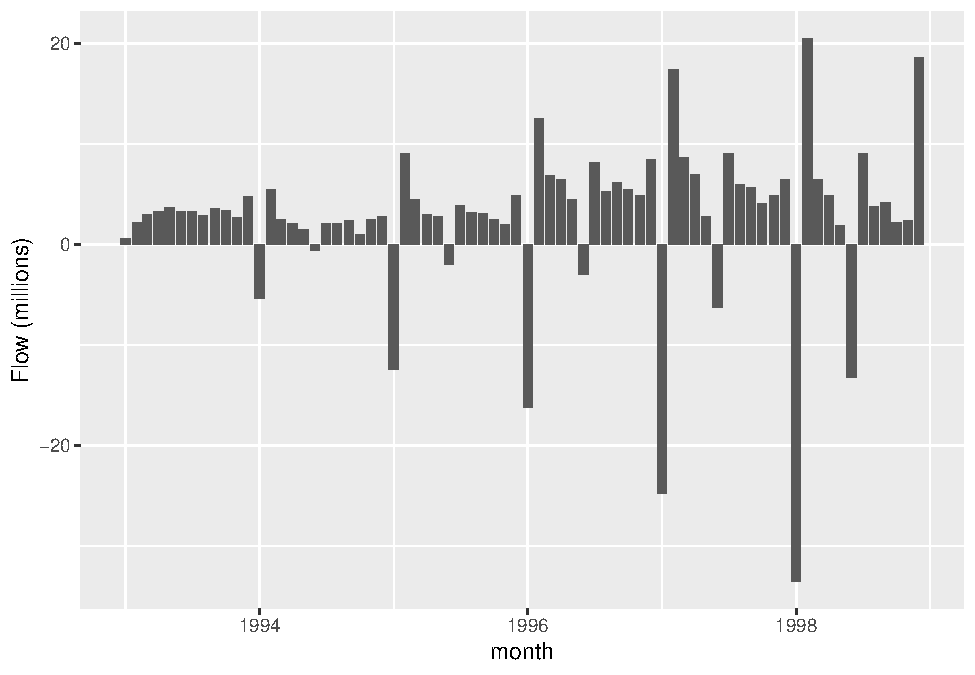
\includegraphics{bookdown_files/figure-latex/unnamed-chunk-37-1.pdf}
\caption{\label{fig:unnamed-chunk-37}Net transactions amount monthly}
\end{figure}

Looking in the types of transactions we can see that the negative cash
flow is caused by a surge in the number of withdrawals.

\begin{figure}
\centering
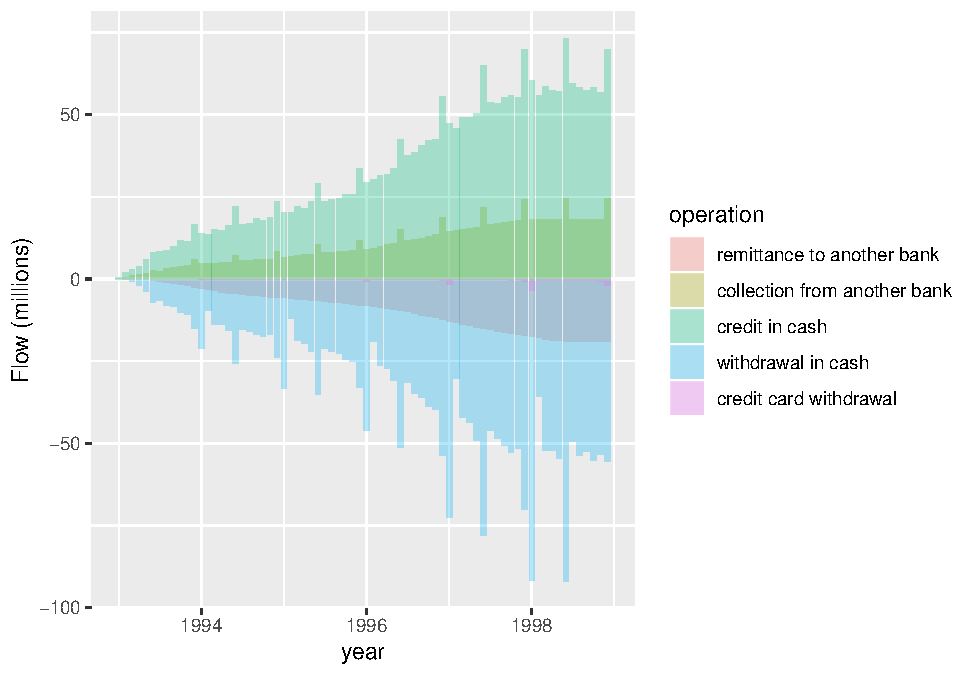
\includegraphics{bookdown_files/figure-latex/unnamed-chunk-38-1.pdf}
\caption{\label{fig:unnamed-chunk-38}Cash Flow Year by Year}
\end{figure}

From the products categorized by the bank we can see that household has
the fastest growth, even though it and the other products are going
through a period of stagnation recently.

\begin{figure}
\centering
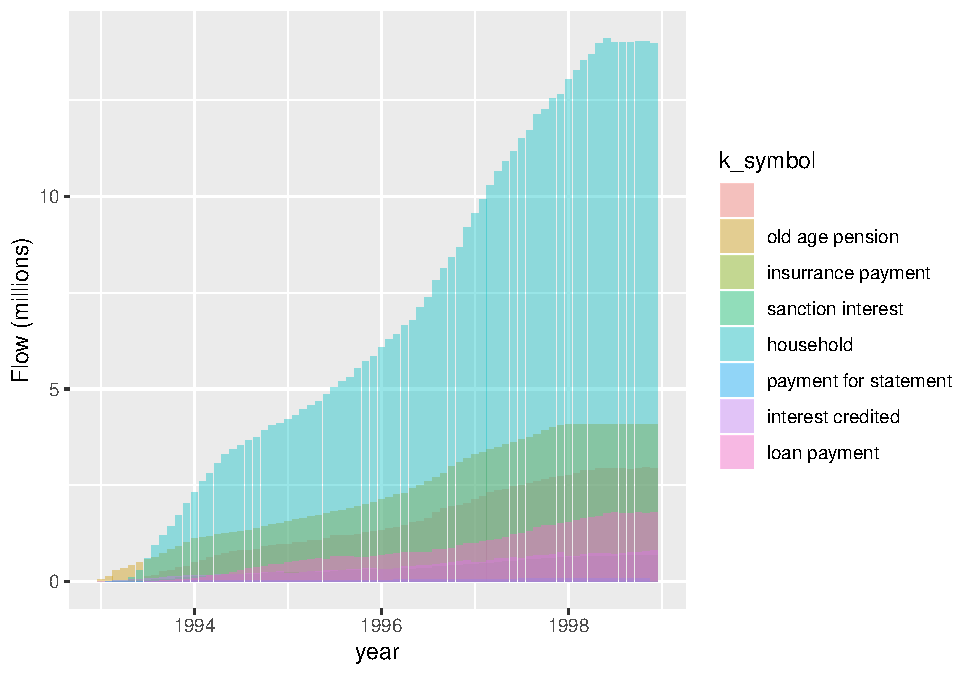
\includegraphics{bookdown_files/figure-latex/unnamed-chunk-39-1.pdf}
\caption{\label{fig:unnamed-chunk-39}Cash Flow Year by Year}
\end{figure}

\chapter{Orders}\label{orders}

\section{Order types}\label{order-types}

From the orders segmented by the bank household stands out as the most
relevant one.

Creating special deals for this type of order may be a good opportunity
for growing the bank but it's important to analyse if there's still a
tendency in this direction. The risk is that this order type was very
significant in the last years due to the economic situation of the
country (from socialism to capitalism) and maybe from now on other order
types will become more relevant for the population.

\begin{figure}
\centering
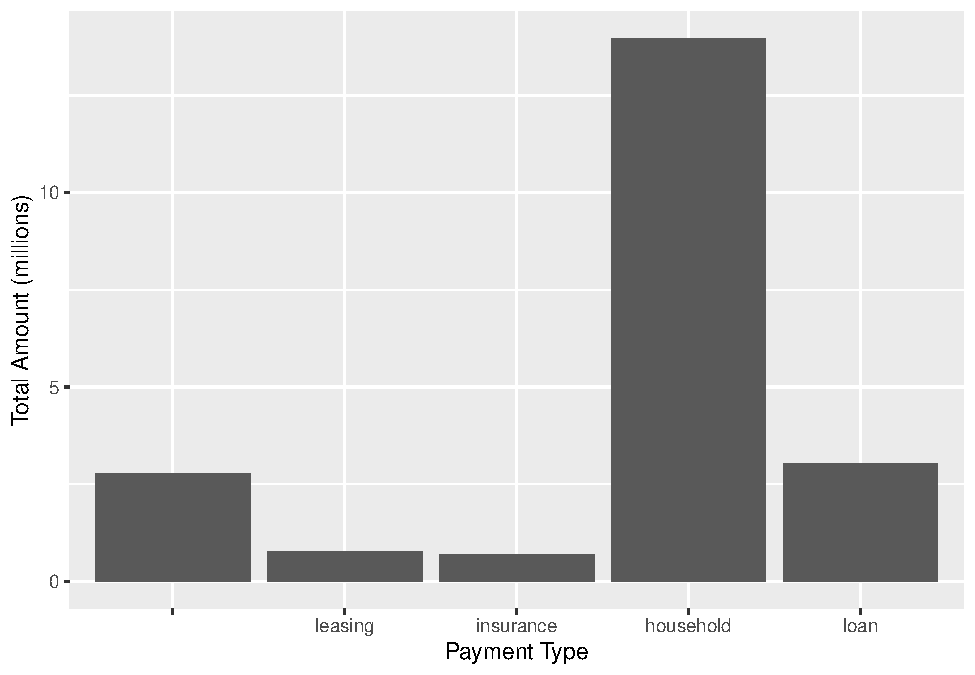
\includegraphics{bookdown_files/figure-latex/unnamed-chunk-41-1.pdf}
\caption{\label{fig:unnamed-chunk-41}Payment Type}
\end{figure}

\chapter{Cards}\label{cards}

\section{Card type}\label{card-type}

The majority of the cards issued by the bank are of the classic type.

Since credit cards are not yet widely used by customers, offering
premium cards can be a good opportunity to encourage their use.

\begin{figure}
\centering
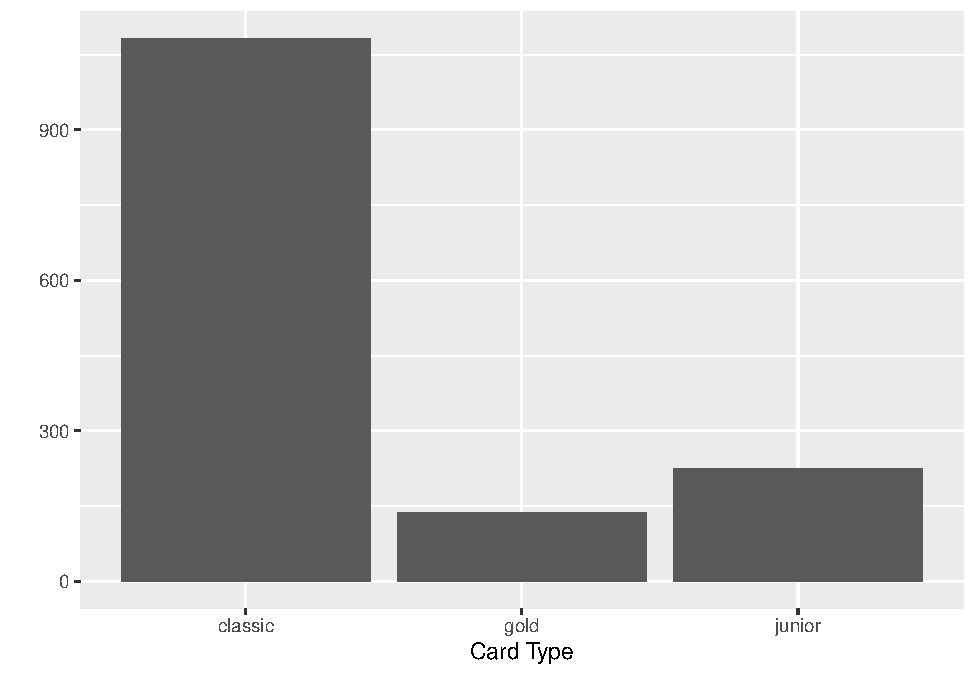
\includegraphics{bookdown_files/figure-latex/unnamed-chunk-42-1.pdf}
\caption{\label{fig:unnamed-chunk-42}Card Type}
\end{figure}

\section{Card type issued by year}\label{card-type-issued-by-year}

There has been an increase in the number of cards issued by the bank
pushed mostly by the classic card.

\begin{figure}
\centering
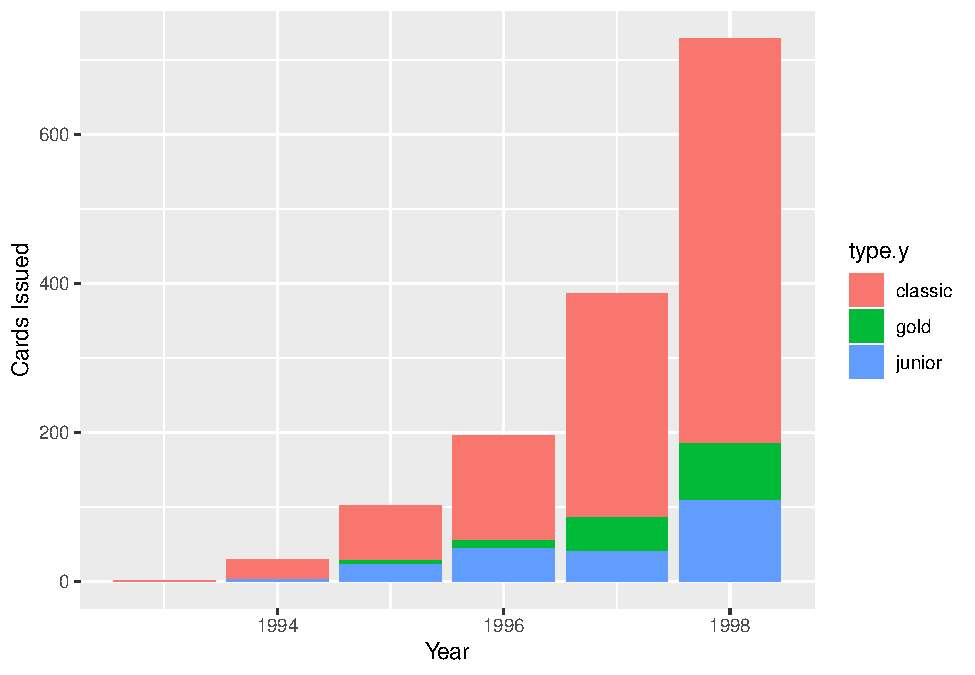
\includegraphics{bookdown_files/figure-latex/unnamed-chunk-43-1.pdf}
\caption{\label{fig:unnamed-chunk-43}Cards issued by date}
\end{figure}

\section{Credit card transactions by
type}\label{credit-card-transactions-by-type}

The growth in the number of credit cards has also been accompanied by a
grow in the number of transactions done by credit card, mostly in the
classic card.

\begin{figure}
\centering
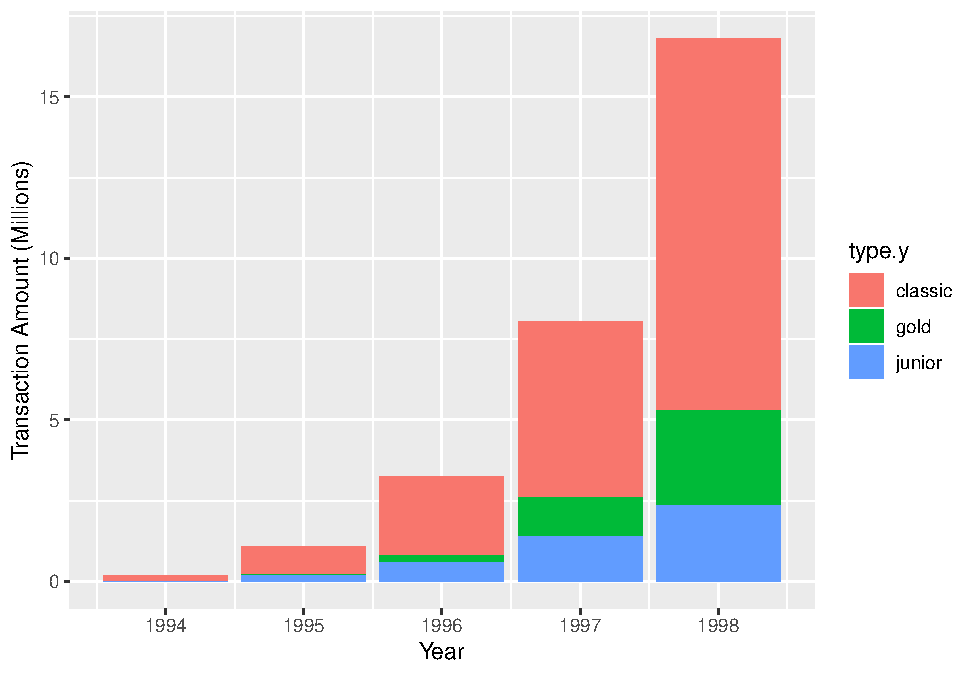
\includegraphics{bookdown_files/figure-latex/unnamed-chunk-44-1.pdf}
\caption{\label{fig:unnamed-chunk-44}Amount of transactions by card type}
\end{figure}

\section{Credit card transactions by
type}\label{credit-card-transactions-by-type-1}

The growth in the number of credit cards has also been accompanied by a
grow in the number of transactions done by credit card, mostly in the
classic card.

\begin{figure}
\centering
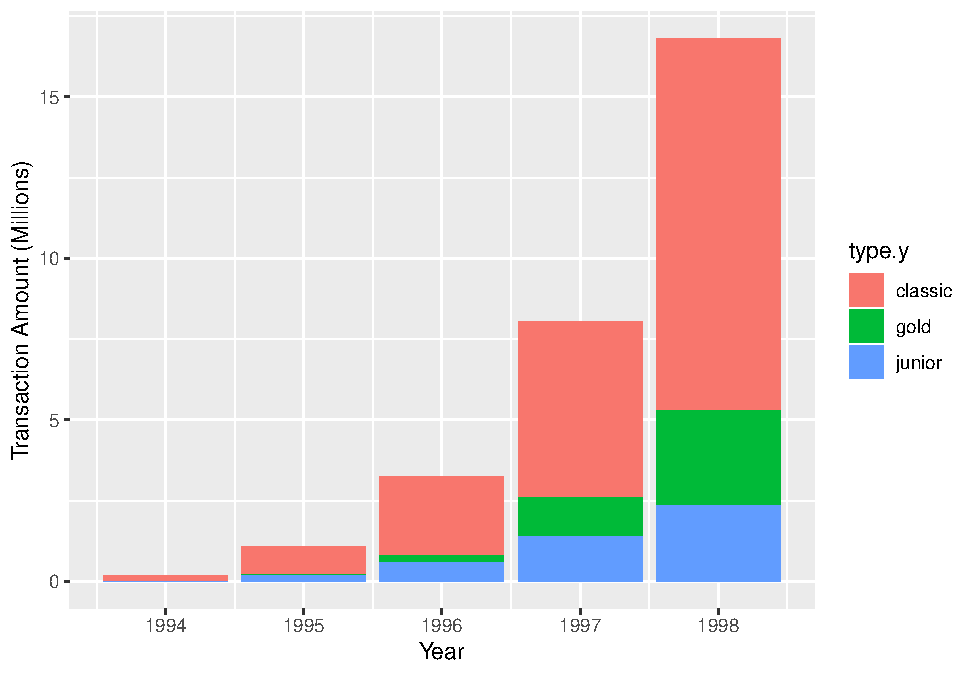
\includegraphics{bookdown_files/figure-latex/unnamed-chunk-45-1.pdf}
\caption{\label{fig:unnamed-chunk-45}Amount of transactions by card type}
\end{figure}

\section{Credit card transactions by
month}\label{credit-card-transactions-by-month}

As it happens with the amount of transactions there is also a spike in
the use of credit cards every year in January, especially amongst the
users of the classic card.

\begin{figure}
\centering
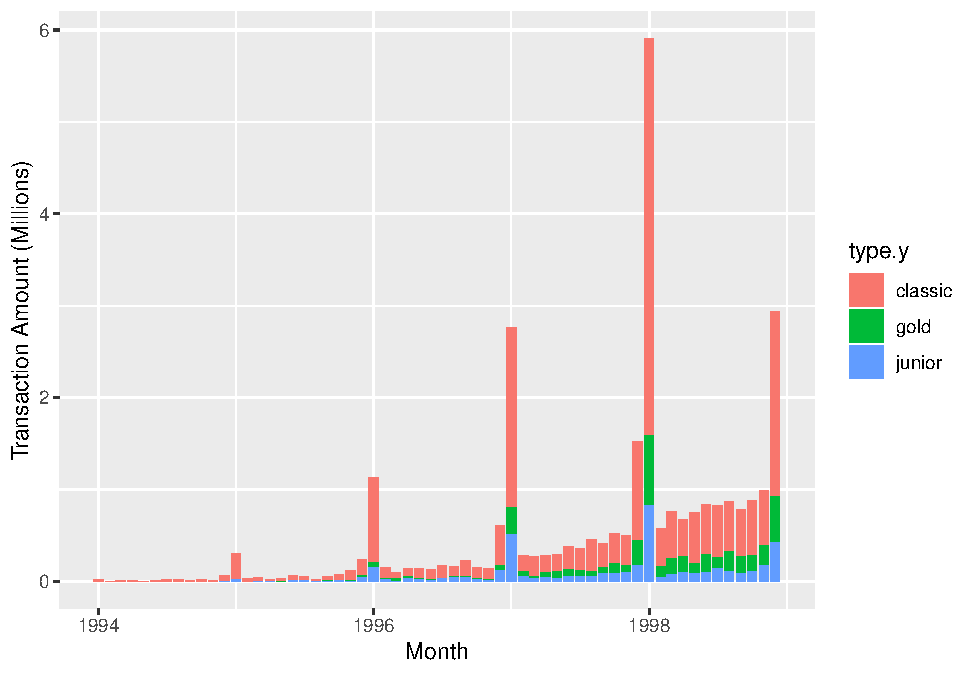
\includegraphics{bookdown_files/figure-latex/unnamed-chunk-46-1.pdf}
\caption{\label{fig:unnamed-chunk-46}Amount of transactions by month}
\end{figure}

\section{Amount of card transactions by
account}\label{amount-of-card-transactions-by-account}

The gold card has a slightly higher volume of transactions per client
then the other cards. Looking at the clients with the classic card we
see that there is a great number of outliers regarding the total of
transactions with the card, those clients could be updated to the gold
card.

\begin{figure}
\centering
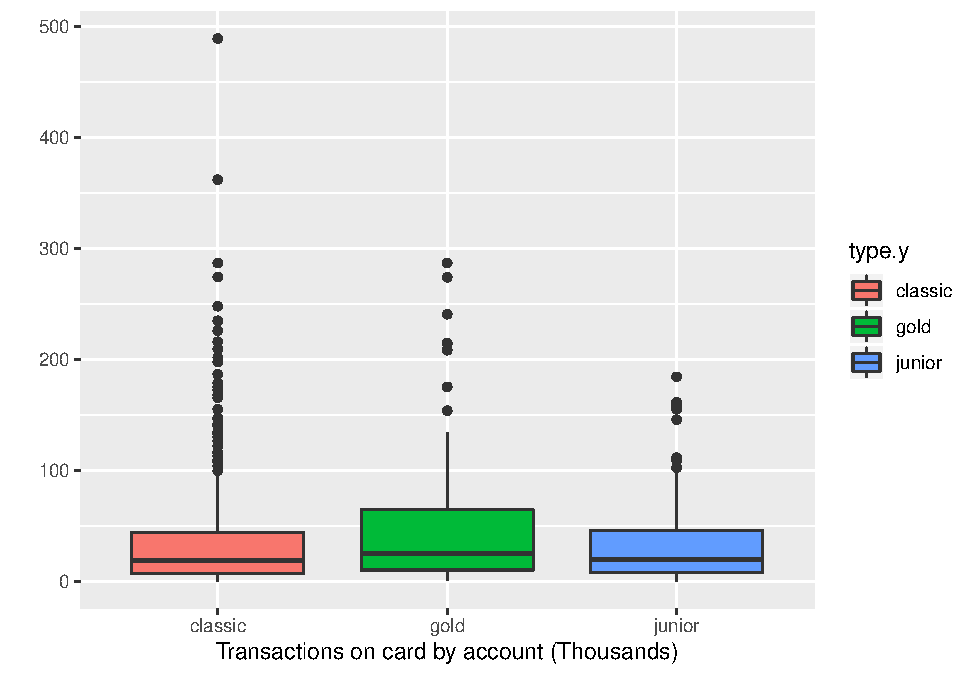
\includegraphics{bookdown_files/figure-latex/unnamed-chunk-47-1.pdf}
\caption{\label{fig:unnamed-chunk-47}Amount of card transactions by account}
\end{figure}

\chapter{Conclusion}\label{conclusion}

The bank has seen growth in customer numbers but there is plenty of room
to grow.

There is still little penetration in the different regions of the Czech
Republic and the economic climate is very conducive to winning more
customers. Recommendation: Focus on growth first in South Moravia, where
population density is high and the bank does not have many clients yet.
Focusing on growth in these regions, we can then expand to the rest of
the country. Risks: It is important to keep in mind the possible risks
of losing room for competitors in other regions.

The bank has a good repayment rate for loans made, especially those with
lower values. Recommendation: Increase the volume of micro credits,
which are performing well and may attract more customers to the bank.
Risks: As we increase the volume, we increase our default risk, so we
need to work directly with the credit bureau to ensure good customer
reviews before lending.

A critical point noticed in the analysis is the large amount of
withdrawals in July and January, leaving the bank balance negative. It
is essential that the bank understands the motivations of customers in
these months, to anticipate and not suffer in these months.
Recommendation: Conduct qualitative customer research to understand this
movement. Based on this, structure action paths to minimize impacts.
Risks: Customers may feel overrun when asked about their movements, so
it is important to drive carefully to avoid dissatisfaction with the
bank.

Finally, we see a growth in the number of cards issued in recent years,
but still with little movement from them. Recommendation: Create more
incentives for credit card use. This can be done by offering more
premium cards and ensuring more credit per user. Risks: Because credit
cards are not yet part of the Czech Republic's culture, we may have a
period of learning how to use the card, which may cause delinquent
invoices.

As next steps, we suggest further analysis and exploration of the above
points.


\end{document}
